% ============================================================
%  BTL2 — Source/2/main.tex
%  Task 2.1: Nhận dạng Thực thể có Tên (Custom NER)
% ============================================================

\section{Tác vụ 2.1: Nhận dạng Thực thể có Tên (Custom NER)}

\subsection{Đặt vấn đề}

Các hệ thống NER tổng quát (spaCy, Stanford NER) không đủ để nhận dạng các thực thể đặc thù trong hợp đồng pháp lý như tỷ lệ phạt, điều khoản bồi thường, hay luật điều chỉnh. Tác vụ này yêu cầu xây dựng và fine-tune mô hình NER chuyên biệt trên domain pháp lý.

\subsection{Schema thực thể}

\begin{table}[H]
    \centering
    \caption{Schema thực thể sử dụng trong BTL2}
    \label{tab:ner_schema}
    \begin{tabularx}{\textwidth}{|l|X|l|}
        \hline
        \textbf{Nhãn} & \textbf{Ý nghĩa} & \textbf{Ví dụ} \\ \hline
        PARTY   & Bên ký kết hợp đồng & \textit{Party A, Employee, Licensor} \\ \hline
        MONEY   & Giá trị tài chính   & \textit{10,000,000 VND, USD 50,000} \\ \hline
        DATE    & Ngày, thời hạn      & \textit{05 May 2024, within 30 days} \\ \hline
        RATE    & Tỷ lệ phần trăm     & \textit{2.5\%, 18\% per annum} \\ \hline
        PENALTY & Điều khoản phạt     & \textit{liquidated damages, penalty} \\ \hline
        LAW     & Luật, văn bản pháp lý & \textit{laws of California, CISG} \\ \hline
    \end{tabularx}
\end{table}

\subsection{Xây dựng Dataset}

\subsubsection{Nguồn dữ liệu}

Dataset NER được xây dựng từ hai nguồn:
\begin{itemize}
    \item \textbf{CUAD Dataset}: Tập hợp đồng thương mại thực tế gồm hơn 500 hợp đồng tiếng Anh, được dùng để trích xuất các đoạn văn phong phú về entity.
    \item \textbf{Synthetic Data}: Các mẫu tổng hợp được sinh bằng LLM (Llama-3.1-8B-Instruct) theo pipeline Delta Operation, đảm bảo span character-level chính xác.
\end{itemize}

\subsubsection{Quy trình annotation}

Pipeline annotation sử dụng kiến trúc \textbf{Delta Operation}:
\begin{enumerate}
    \item LLM nhận văn bản và trả về danh sách thao tác JSON (thêm/xóa entity) thay vì tagged text.
    \item Python thực hiện căn chỉnh span xác định (deterministic span alignment) để tránh offset drift.
    \item Pruner stage kiểm tra tính hợp lệ: loại bỏ span trùng lắp, entity nằm ngoài text, nhãn mơ hồ.
\end{enumerate}

\subsubsection{Thống kê dataset}

\begin{table}[H]
    \centering
    \caption{Phân bố dataset NER sau annotation}
    \label{tab:ner_dataset}
    \begin{tabular}{|l|r|r|}
        \hline
        \textbf{Nhãn} & \textbf{Số entity} & \textbf{Tỷ lệ (\%)} \\ \hline
        PARTY   & -- & -- \\ \hline
        MONEY   & -- & -- \\ \hline
        DATE    & -- & -- \\ \hline
        RATE    & -- & -- \\ \hline
        PENALTY & -- & -- \\ \hline
        LAW     & -- & -- \\ \hline
        \textbf{Tổng mẫu} & \textbf{308} & \textbf{100} \\ \hline
    \end{tabular}
\end{table}

\textit{Lưu ý: Phân bố chi tiết từng nhãn sẽ được điền sau khi chạy script thống kê.}

\subsection{Mô hình và Huấn luyện}

\subsubsection{Kiến trúc}

Mô hình được fine-tune từ \texttt{dslim/bert-base-NER} -- phiên bản BERT-base đã được pre-train sơ bộ trên CoNLL-2003 NER task. Lớp phân loại token được thay thế bằng lớp mới với 7 nhãn (bao gồm \texttt{O}).

\subsubsection{Token Alignment}

Sử dụng \texttt{return\_offsets\_mapping=True} của HuggingFace tokenizer để ánh xạ character-level span sang token-level labels. Token nằm trong $[\text{start}, \text{end})$ của entity được gán nhãn tương ứng; token đặc biệt (\texttt{[CLS]}, \texttt{[SEP]}, padding) được bỏ qua.

\subsubsection{Cấu hình huấn luyện}

\begin{table}[H]
    \centering
    \caption{Siêu tham số huấn luyện NER}
    \label{tab:ner_hyperparams}
    \begin{tabular}{|l|r|}
        \hline
        \textbf{Tham số} & \textbf{Giá trị} \\ \hline
        Base model       & \texttt{dslim/bert-base-NER} \\ \hline
        Max sequence length & 128 \\ \hline
        Batch size       & 8 \\ \hline
        Learning rate    & 3e-5 \\ \hline
        Optimizer        & AdamW \\ \hline
        Scheduler        & Linear warmup \\ \hline
        Epochs           & 10 \\ \hline
        Train / Val / Test split & 80\% / 10\% / 10\% \\ \hline
    \end{tabular}
\end{table}

\subsection{Kết quả}

\subsubsection{Lịch sử huấn luyện}

Hình~\ref{fig:ner_training} thể hiện train loss và validation loss qua 10 epochs.

\begin{figure}[H]
    \centering
    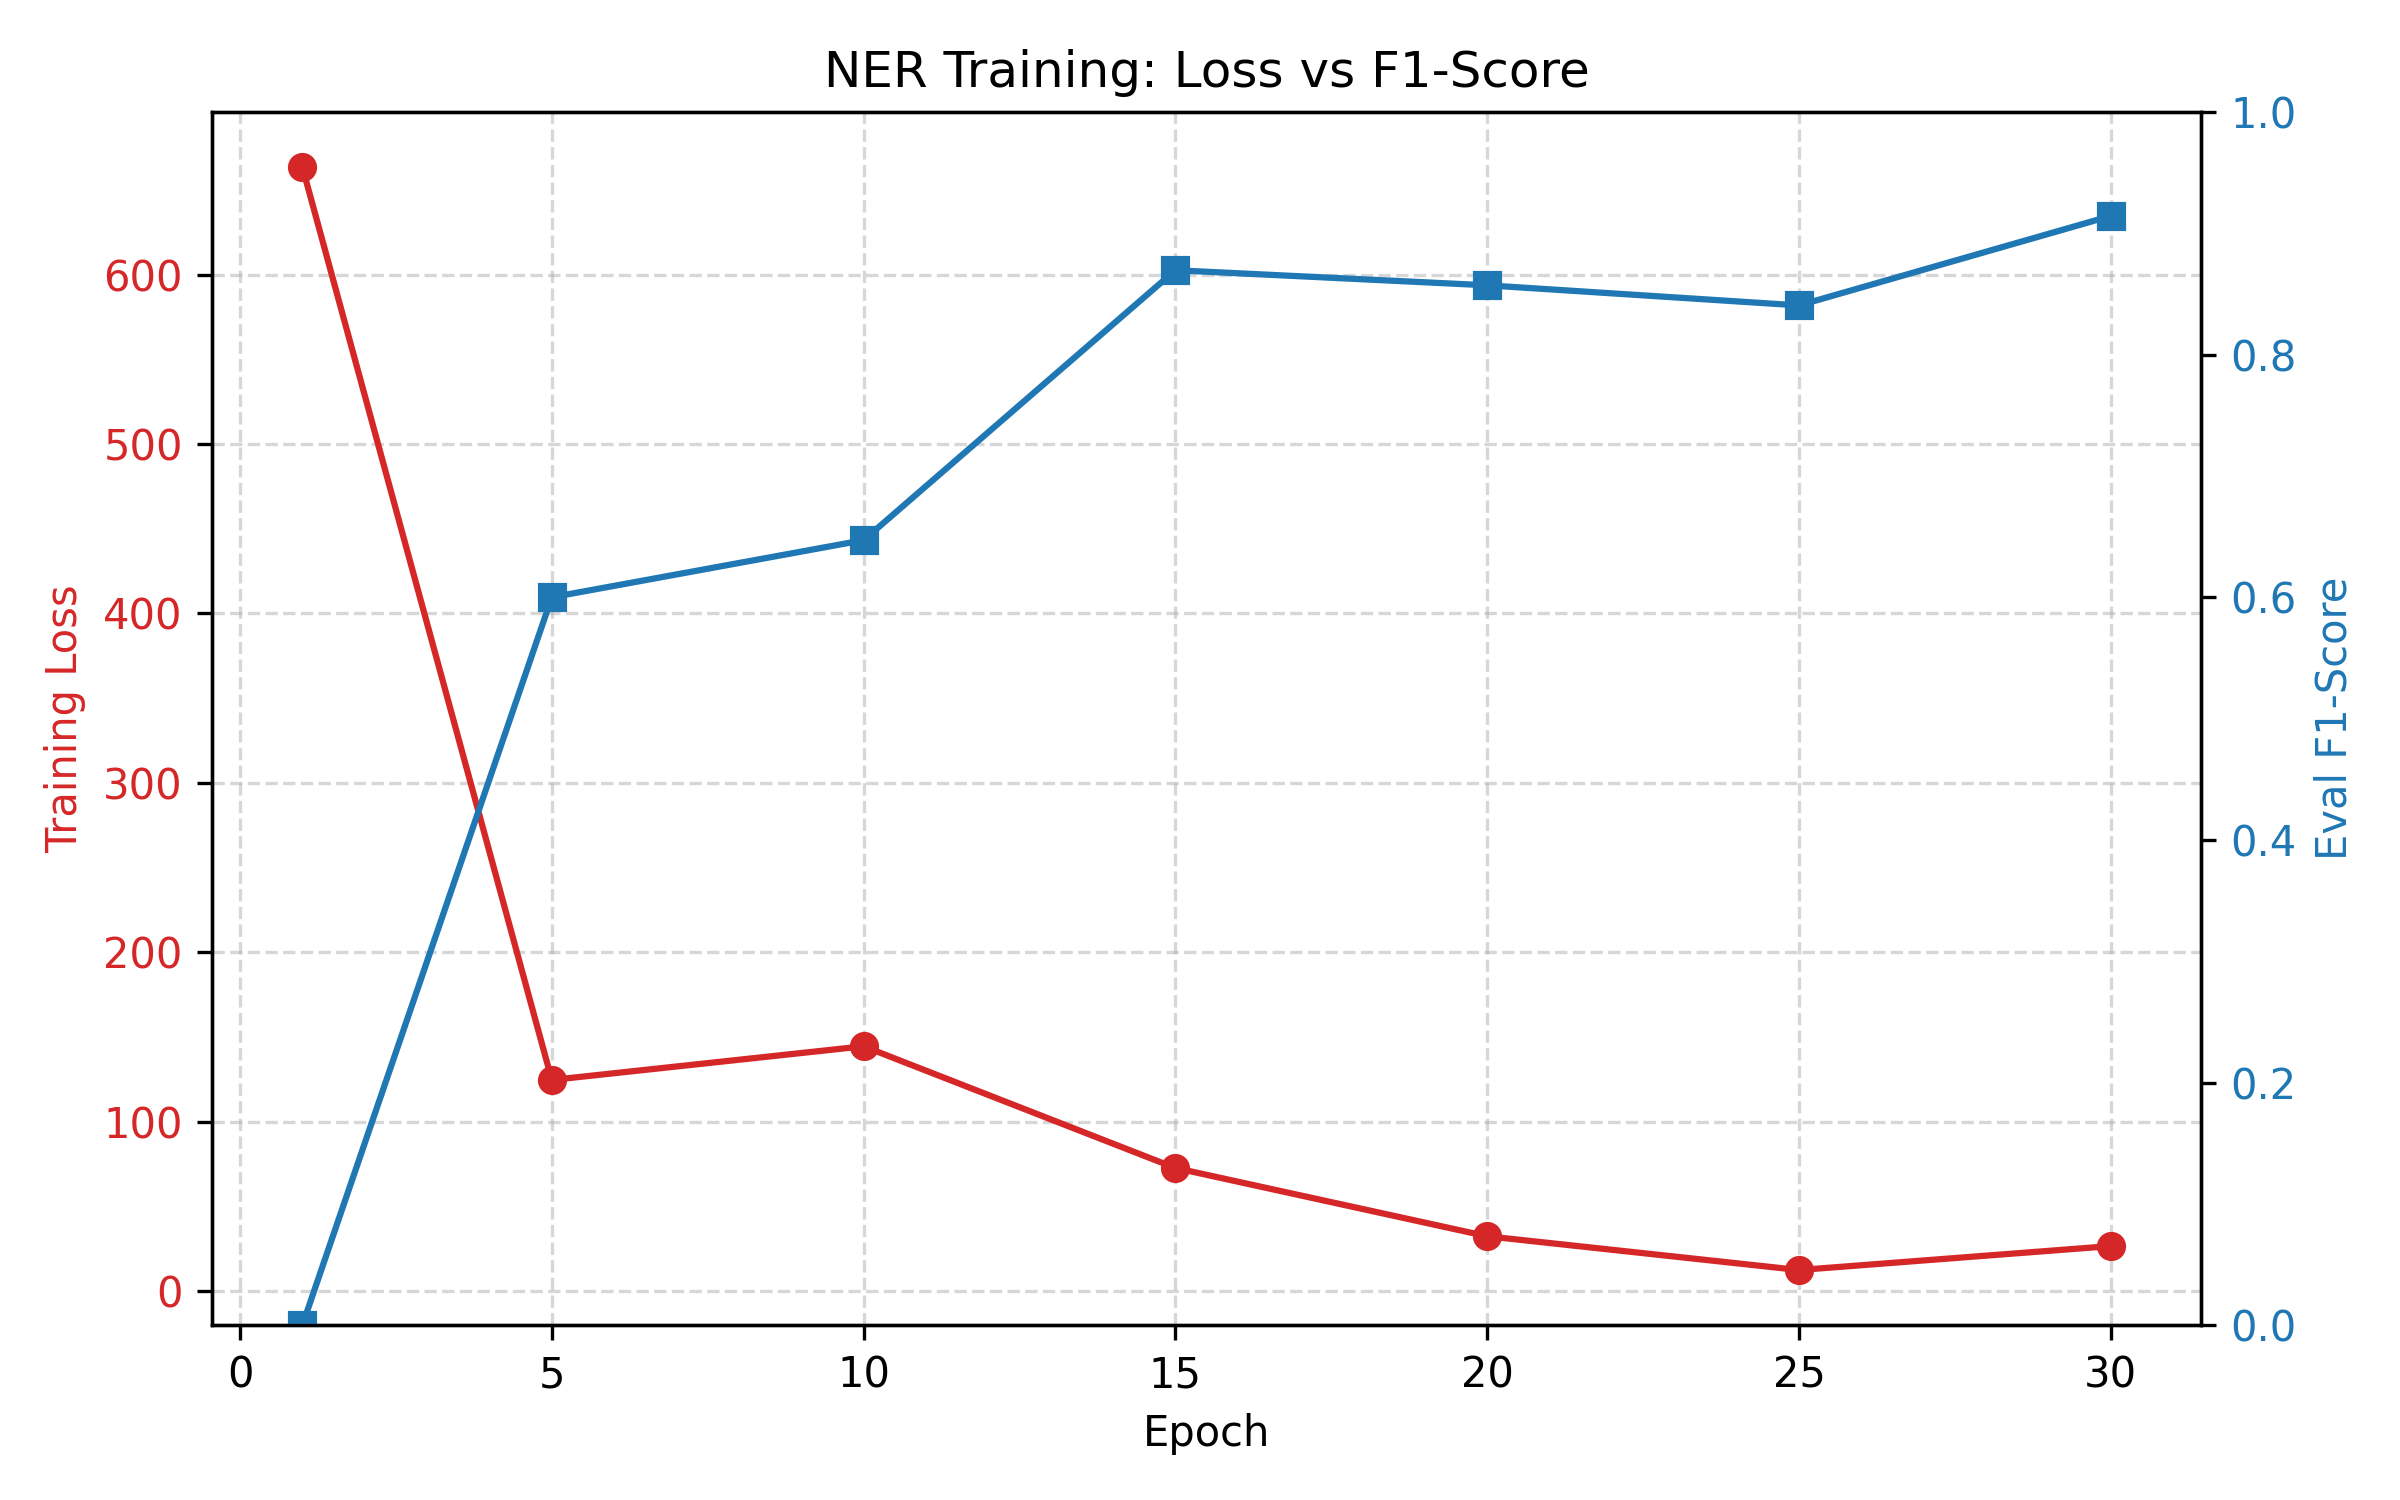
\includegraphics[width=0.85\textwidth]{../BTL2/report_assets/ner_training_history.png}
    \caption{Lịch sử Train Loss và Validation Loss của mô hình NER qua 10 epochs}
    \label{fig:ner_training}
\end{figure}

\subsubsection{Kết quả phân loại}

\begin{table}[H]
    \centering
    \caption{Kết quả classification report trên tập test NER}
    \label{tab:ner_results}
    \begin{tabular}{|l|r|r|r|r|}
        \hline
        \textbf{Nhãn} & \textbf{Precision} & \textbf{Recall} & \textbf{F1-score} & \textbf{Support} \\ \hline
        O       & -- & -- & -- & -- \\ \hline
        PARTY   & -- & -- & -- & -- \\ \hline
        MONEY   & -- & -- & -- & -- \\ \hline
        DATE    & -- & -- & -- & -- \\ \hline
        RATE    & -- & -- & -- & -- \\ \hline
        PENALTY & -- & -- & -- & -- \\ \hline
        LAW     & -- & -- & -- & -- \\ \hline
        \textbf{Weighted avg} & -- & -- & -- & -- \\ \hline
    \end{tabular}
\end{table}

\textit{Lưu ý: Kết quả sẽ được điền sau khi chạy \texttt{python src/ner.py -{}-mode all}.}

\subsubsection{Ví dụ đầu ra NER}

\begin{table}[H]
    \centering
    \caption{Một số ví dụ kết quả NER trên tập test}
    \label{tab:ner_examples}
    \begin{tabularx}{\textwidth}{|X|l|l|}
        \hline
        \textbf{Đoạn văn bản} & \textbf{Thực thể} & \textbf{Nhãn} \\ \hline
        \textit{This Agreement shall be governed by the laws of the State of \textbf{California}} & California & LAW \\ \hline
        \textit{...governed by the laws of \textbf{Delaware}} & Delaware & LAW \\ \hline
        \textit{...governed by the laws of \textbf{Ontario, Canada}} & Ontario, Canada & LAW \\ \hline
    \end{tabularx}
\end{table>

\begin{figure}[H]
    \centering
    % PLACEHOLDER: Confusion matrix NER (cần sinh ra khi chạy evaluate)
    \fbox{\parbox{0.7\textwidth}{\centering\vspace{2cm}
    \textbf{[PLACEHOLDER: NER Confusion Matrix]}\\
    \small Sinh ra khi chạy: \texttt{python src/ner.py -{}-mode all}\\
    Lưu tại: \texttt{models/ner\_model/test\_metrics.txt}\\
    \vspace{2cm}}}
    \caption{Confusion matrix của mô hình NER trên tập test}
    \label{fig:ner_confusion}
\end{figure}

\subsection{Nhận xét}

\begin{itemize}
    \item Nhãn \textbf{LAW} và \textbf{PARTY} thường được nhận dạng tốt do pattern rõ ràng và xuất hiện nhiều trong training data.
    \item Nhãn \textbf{PENALTY} và \textbf{RATE} khó hơn vì context đa dạng và số mẫu ít hơn trong dataset.
    \item Token alignment với offset mapping giúp tránh lỗi căn chỉnh khi BERT WordPiece tách từ.
\end{itemize}
